\documentclass{beamer}

\usepackage[utf8]{inputenc}
\usepackage{tikz}
\usetikzlibrary{mindmap,trees,shadows}

\mode<presentation>
{
  \usetheme{Warsaw}
  
  \setbeamercovered{transparent}
}

\newcounter{saveenumi}
\newcommand{\seti}{\setcounter{saveenumi}{\value{enumi}}}
\newcommand{\conti}{\setcounter{enumi}{\value{saveenumi}}}

\resetcounteronoverlays{saveenumi}

\AtBeginSubsection[]
{
  \begin{frame}<beamer>{Outline}
    \tableofcontents[currentsection,currentsubsection]
  \end{frame}
}


% If you wish to uncover everything in a step-wise fashion, uncomment
% the following command: 

\beamerdefaultoverlayspecification{<+->}


\title[The category of representations]
{The category of representations of a concrete category as a functor category}

\author{Tibor Gr{\"u}n}

%\date{October 30, 2020} % date of printed version
%\date{November 3, 2020} % date of submission
\date{November 16, 2020} % date of seminar presentation
\begin{document}

  % Keys to support piece-wise uncovering of elements in TikZ pictures:
  % \node[visible on=<2->](foo){Foo}
  % \node[visible on=<{2,4}>](bar){Bar}   % put braces around comma expressions
  %
  % Internally works by setting opacity=0 when invisible, which has the 
  % adavantage (compared to \node<2->(foo){Foo} that the node is always there, hence
  % always consumes space plus that coordinate (foo) is always available.
  %
  % The actual command that implements the invisibility can be overriden
  % by altering the style invisible. For instance \tikzsset{invisible/.style={opacity=0.2}}
  % would dim the "invisible" parts. Alternatively, the color might be set to white, if the
  % output driver does not support transparencies (e.g., PS) 
  %
  \tikzset{
    invisible/.style={opacity=0},
    visible on/.style={alt={#1{}{invisible}}},
    alt/.code args={<#1>#2#3}{%
      \alt<#1>{\pgfkeysalso{#2}}{\pgfkeysalso{#3}} % \pgfkeysalso doesn't change the path
    },
  }

\begin{frame}
  \titlepage
\end{frame}

\begin{frame}
\frametitle{Overview}
\begin{tikzpicture}[mindmap, concept color=gray!50, font=\sf, text=white]

  \tikzstyle{level 1 concept}+=[font=\sf, sibling angle=90,level distance = 30mm]

  \node[concept,scale=0.7] {Gedächtnis}
    [clockwise from=135]
        child[concept color=orange, visible on=<2->]{ node[concept,scale=0.7]{Musik} } 
        child[concept color=orange, visible on=<3->]{ node[concept,scale=0.7]{Kunst} } 
        child[concept color=orange, visible on=<4->]{ node[concept,scale=0.7]{Mathematik} } 
        child[concept color=orange, visible on=<5->]{ node[concept,scale=0.7]{Seltenere} };

\end{tikzpicture}

\end{frame}

\begin{frame}

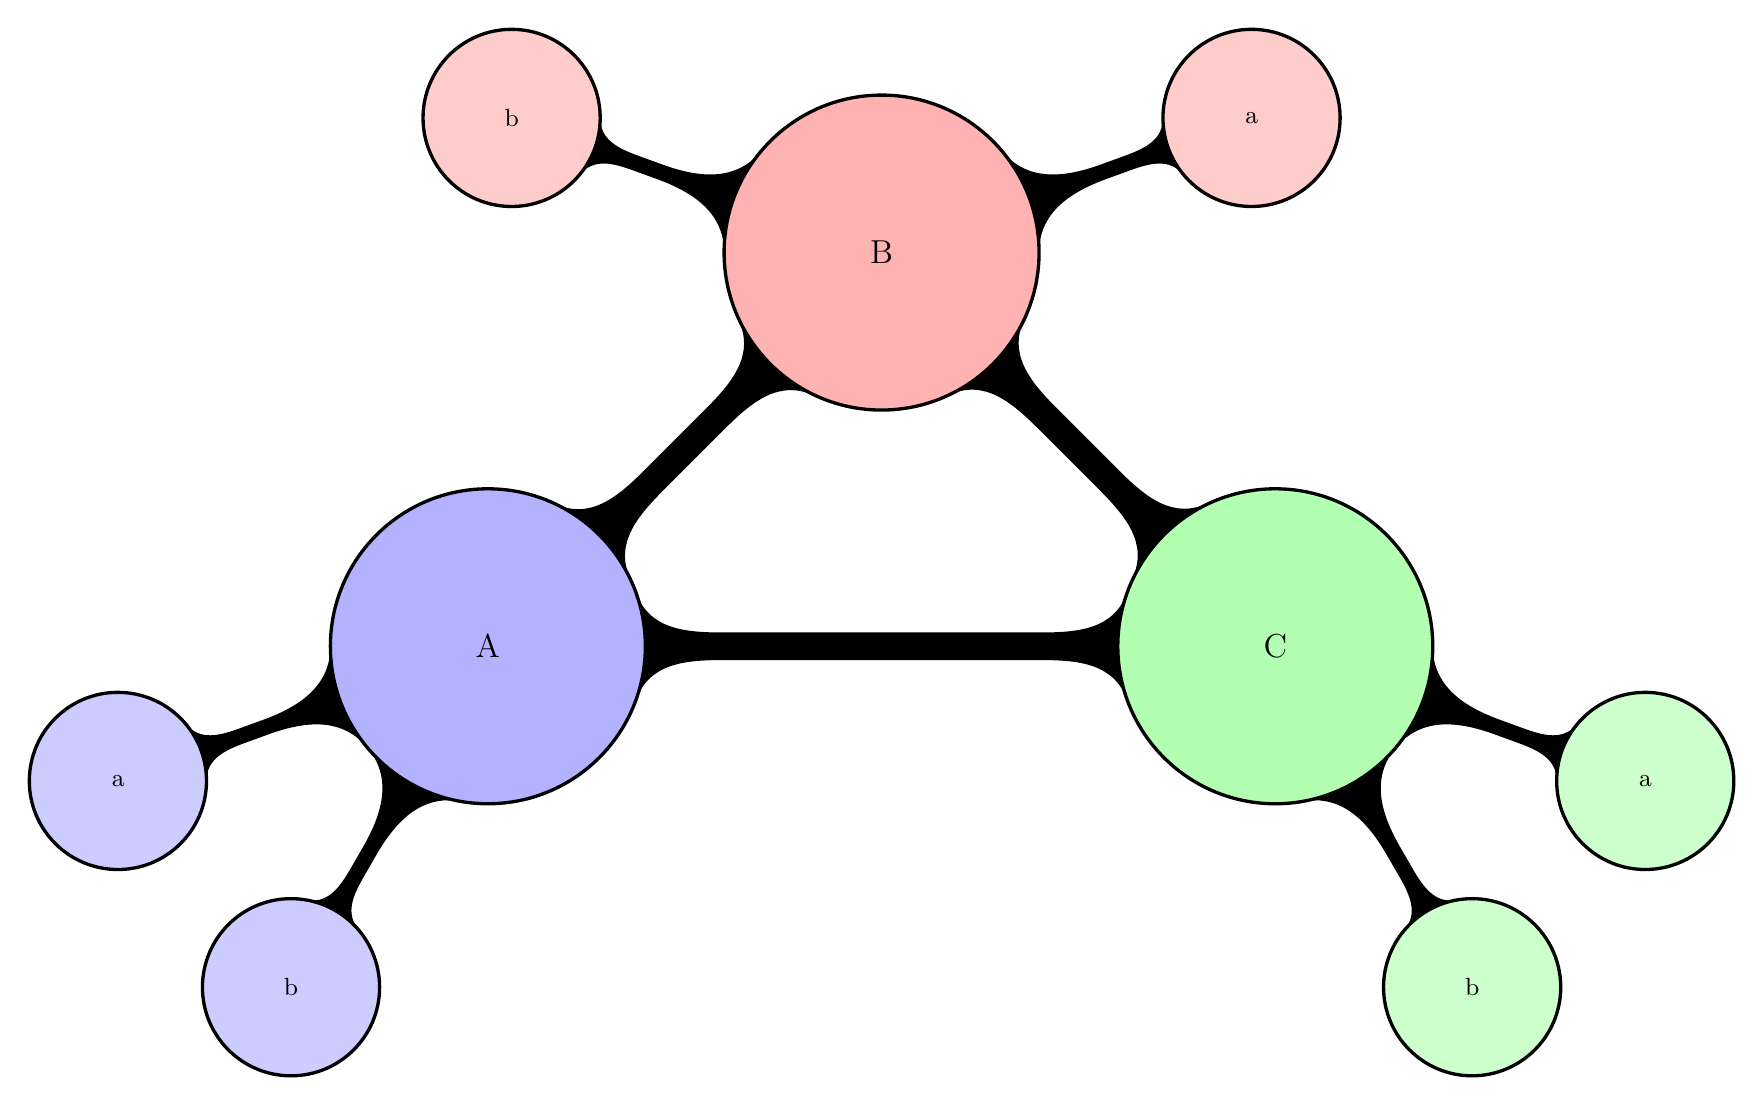
\begin{tikzpicture}[mindmap,concept color=black]

  \node[concept,fill=blue!30] (A) at (0,0) {A}
   child[grow=200] {node[concept,fill=blue!20] (Aa) {a}}
   child[grow=240] {node[concept,fill=blue!20] (Ab) {b}};

  \node[concept,fill=red!30] (B) at (5,5) {B}
   child[grow=20] {node[concept,fill=red!20] (Ba) {a}}
   child[grow=160] {node[concept,fill=red!20] (Bb) {b}};

  \node[concept,fill=green!30] (C) at (10,0) {C}
   child[grow=340] {node[concept,fill=green!20] (Ca) {a}}
   child[grow=300] {node[concept,fill=green!20] (Cb) {b}};

  \path
   (A) to[circle connection bar] (B)
   (B) to[circle connection bar] (C) 
   (A) to[circle connection bar] (C);

\end{tikzpicture}

\end{frame}


\section{Menschen}

Wie bin ich zu dieser Arbeit gekommen?

Sebastians entwickeln CAP.

Peter Webb entwickelt catreps in GAP. Findet CAP.

Meine Aufgabe ist es, die Funktionalität von Peter Webbs catreps in CAP
zu verwirklichen als Paket CatReps. Dabei wird hauptsächlich FunctorCategories
verwendet.

QPA2 mit Kamahl war bevor wir AsFpCategory geschrieben hatten die Schnittstelle zwischen
Konkreter Kategorie und abstraktem Algebroid: nämlich die Pfad-Algebra. Daraus ergab sich
überhaupt erst das Kapitel 4 zu Algebra und Algebroid.


\section{Direct sum decomposition}

\subsection{Morphisms between representations}

\begin{frame}
Calculating the External Hom between two representations.
\end{frame}

\section{Finding invariants for representations}

\subsection{Another Jupyter-Notebook example}

\begin{frame}
Representations with the same image on all objects.
\end{frame}



% Motivation
Wrap Peter Webb's catreps into a CAP package CatReps based on the package FunctorCategories.

Ohne Peter Webbs catreps gäbe es meine Arbeit nicht. Ebensowenig ohne CAP.

Meine Arbeit ist die Umsetzung von catreps in CAP und homalg. Insbesondere wird für
Matrizen und Ringe nicht mehr auf die internen Datenstrukturen von Gap zugegriffen, sondern
durch effizientere Datenstrukturen in homalg.

Dies ermöglicht es, 

% Zusammenfassung



% Beispiele

Limitations: Categories with endomorphism monoids that are not explicitly cyclic
can not be represented by our method. This means we can't look at representations
for groups that are not explicitly cyclic, like the

Klein four group: V = {(), (1,2)(3,4), (1,3)(2,4), (1,4)(2,3) }

The first constructions pose no problems yet:

V := ConcreteCategoryForCAP( [ [2,1,4,3], [2,1,4,3], [3,4,1,2], [4,3,2,1] ] );
> A finite concrete category

qV := RightQuiverFromConcreteCategory( V );
> q(1)[a:1->1,b:1->1,c:1->1]

but we get an error as soon as we want to calculate the endomorphism relations:

rel := RelationsOfEndomorphisms( V );
> Error, we assume at most 1 generating endomorphism per vertex

And since these relations are essential going forward and other algorithms rely on it,
we can't go further with this example.

When we are representing groups, we therefore can only work with cyclic groups.

C4 := ConcreteCategoryForCAP( [ [2,3,4,1] ] );
> A finite concrete category

fpC := AsFpCategory( C4 );
> Monoid generated by the right quiver q(1)[a:1->1] with relations [ a*a*a*a = 1 ]


C6 := ConcreteCategoryForCAP( [ [2,3,4,5,6,1] ] );
















\end{document}